% =============================================================
%  Chapitre 3 — Conception
% =============================================================
\chapter{Conception}

\section*{Introduction}
Ce chapitre présente les choix d'architecture et de conception retenus
pour Telnet Test Manager. On y trouve l'architecture générale, les
diagrammes de classes et de séquence des cas d'utilisation principaux,
et le modèle de données MongoDB.

% -----------------------------------------------------------------
\section{Architecture générale de l'application}
% -----------------------------------------------------------------

\subsection{Architecture globale du système}

\begin{figure}[H]
  \centering
  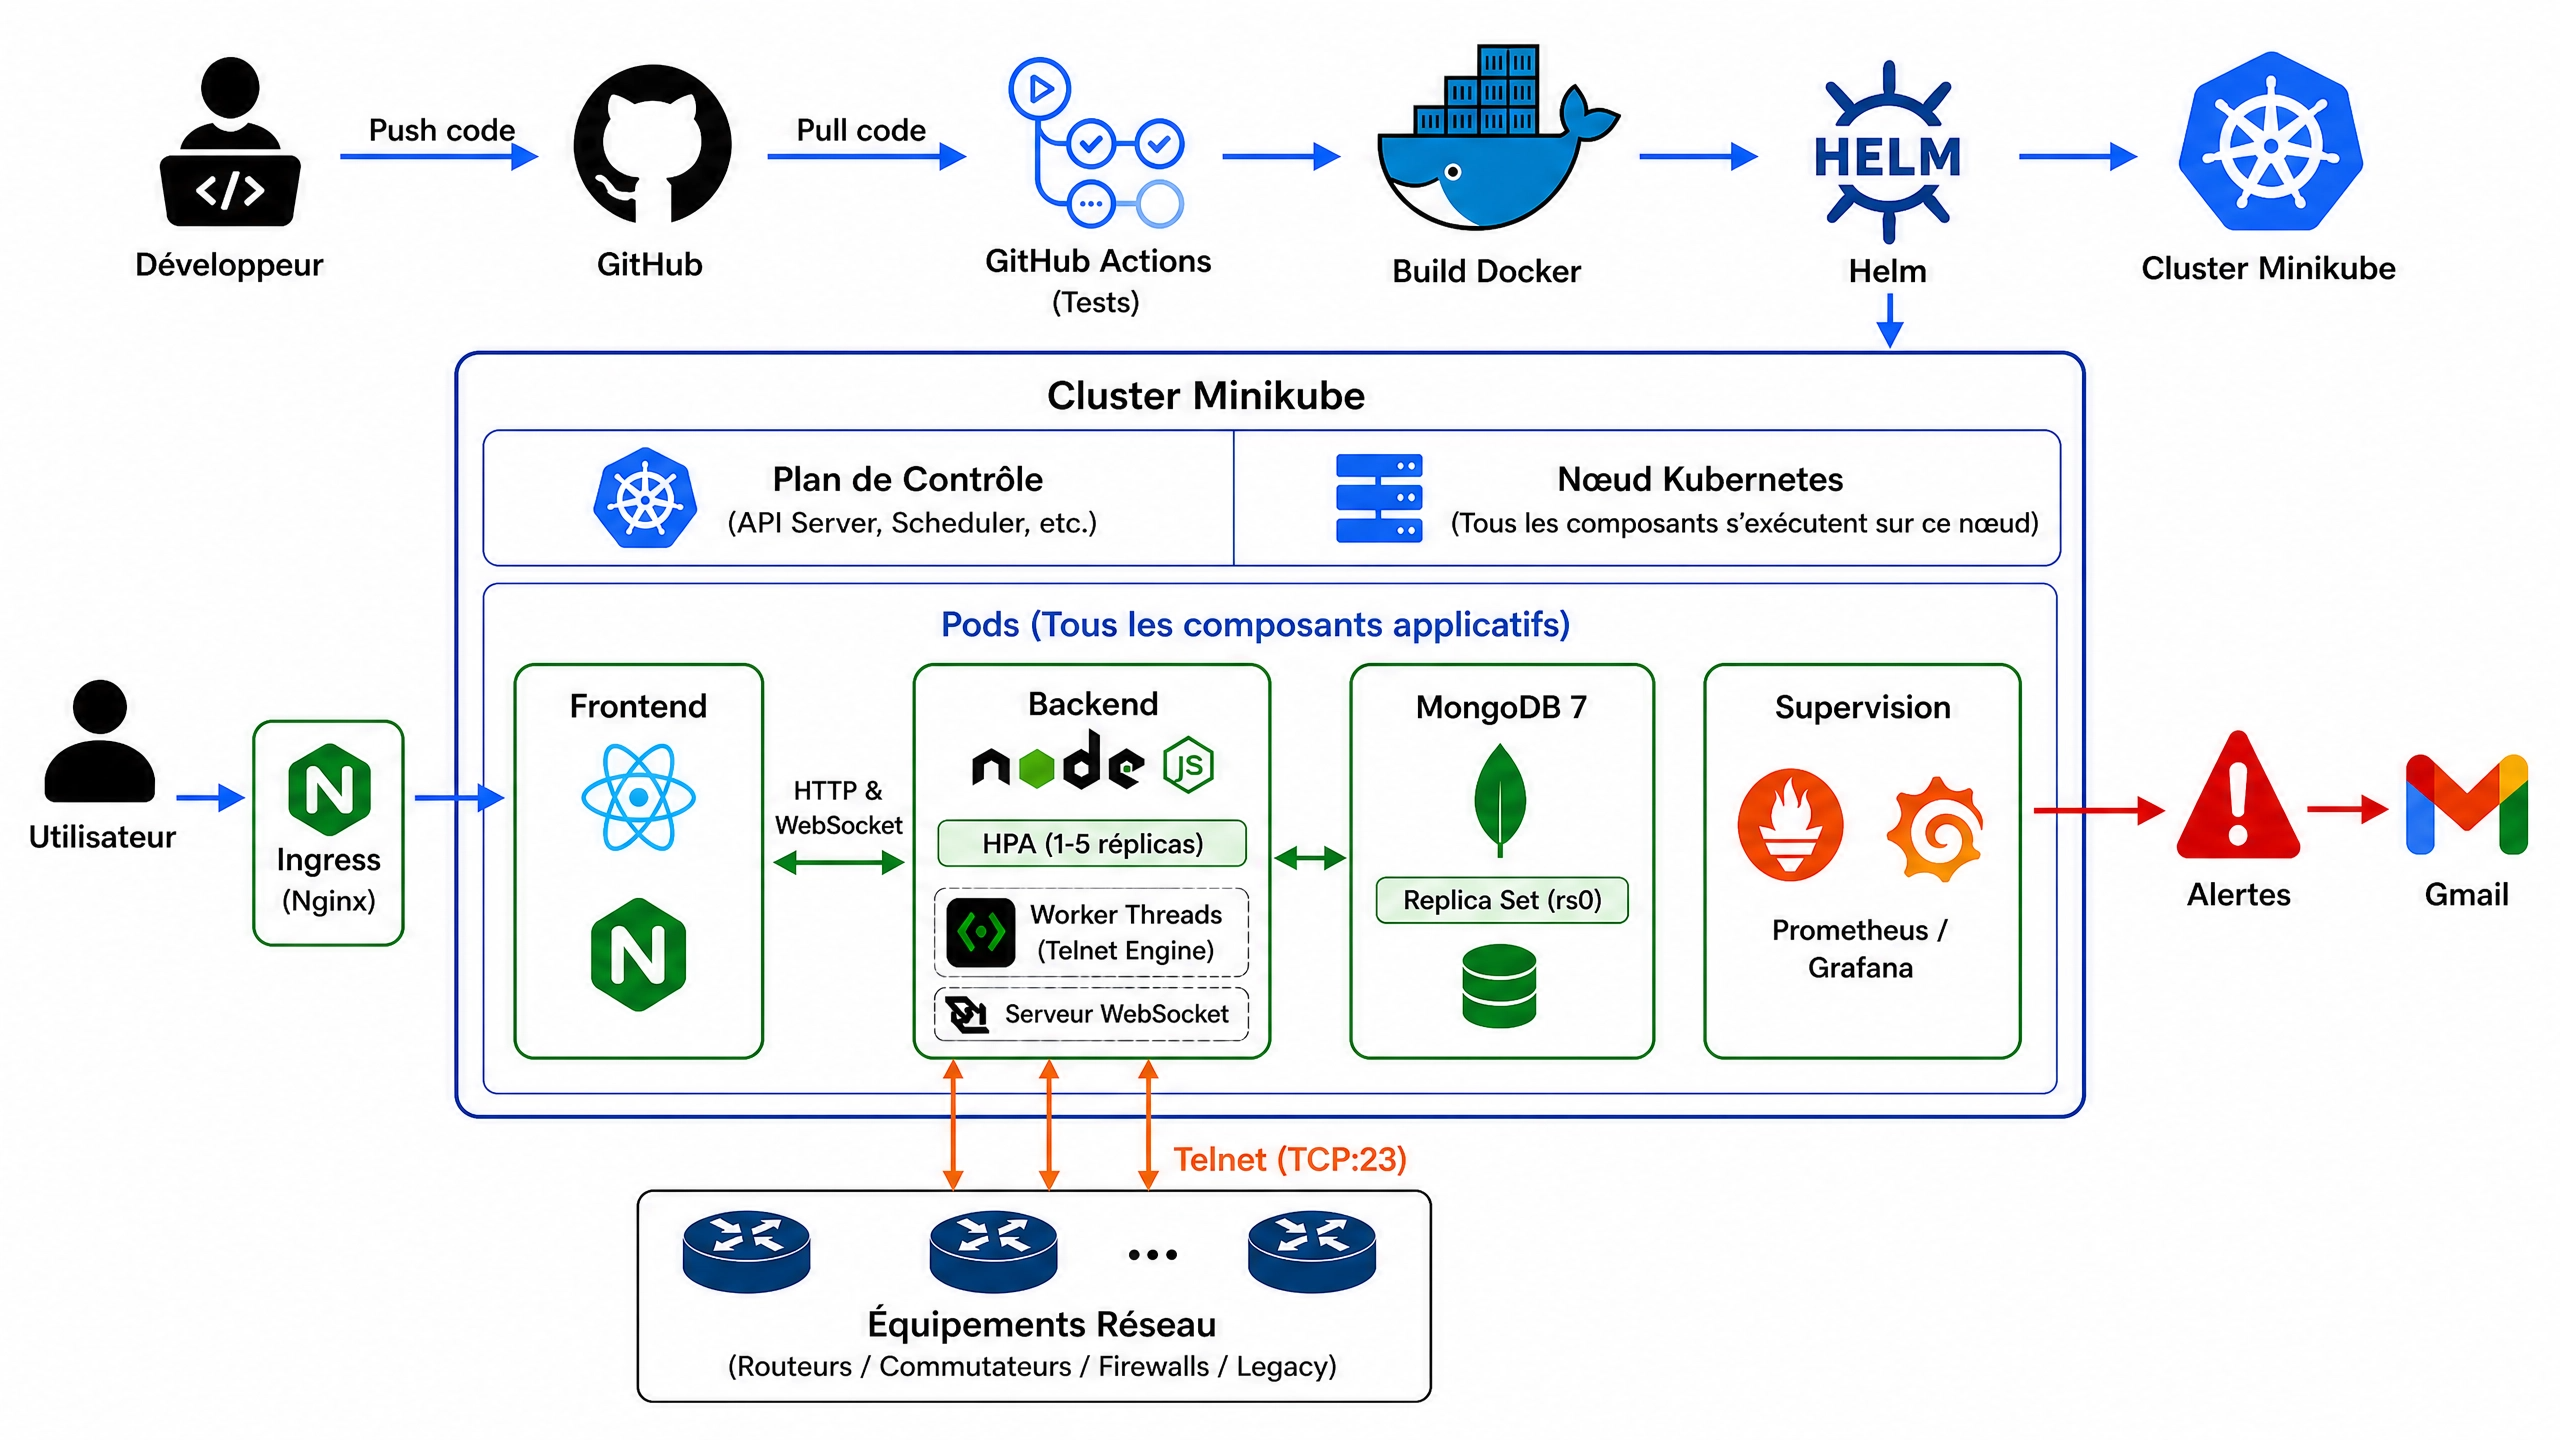
\includegraphics[width=\textwidth]{images/architecture_globale_finale}
  \caption{Architecture globale du système Telnet Test Manager}
  \label{fig:archi_globale}
\end{figure}

\subsection{Architecture N-tiers}

L'application est organisée selon une architecture \textbf{N-tiers} qui
sépare les responsabilités en couches distinctes~:

\begin{figure}[H]
  \centering
  \includegraphics[width=\textwidth]{"images/architecture N tiers"}
  \caption{Architecture N-tiers de l'application Telnet Test Manager}
  \label{fig:archi_ntiers}
\end{figure}

\subsection{Clean Architecture}

Le backend suit les principes de la \textbf{Clean Architecture}
\cite{martin2017clean}. L'idée centrale est simple~: les règles métier
ne dépendent d'aucun détail d'infrastructure. Les dépendances ne
peuvent pointer que \textit{vers l'intérieur}~:

\begin{figure}[H]
  \centering
  \includegraphics[width=0.75\textwidth]{"images/clean architecture"}
  \caption{Diagramme des couches de la Clean Architecture du backend}
  \label{fig:clean_archi}
\end{figure}

% -----------------------------------------------------------------
\section{Choix technologiques}
% -----------------------------------------------------------------

\subsubsection*{Développement Backend}

\subsection{Node.js / Express.js}

\textbf{Node.js} (v20 LTS) est un environnement d'exécution JavaScript
côté serveur basé sur le moteur V8. Son modèle non bloquant et le
support natif des Worker Threads le rendent bien adapté à un serveur
Telnet concurrent. \textbf{Express.js} (v4.18) structure l'application
en routes, middlewares et contrôleurs.

\begin{figure}[H]
  \centering
  
\includegraphics[width=0.28\textwidth]{images/nodejs}
  \caption{Logo Node.js / Express.js}
  \label{fig:logo_node}
\end{figure}

\subsection{MongoDB / Mongoose}

\textbf{MongoDB~7} est une base de données orientée documents (\gls{nosql}).
Son schéma flexible convient bien aux structures variables des résultats
de tests Telnet. \textbf{Mongoose~9} apporte la validation des schémas
et les middlewares d'accès aux données.

\begin{figure}[H]
  \centering
  
\includegraphics[width=0.28\textwidth]{images/mongodb}
  \caption{Logo MongoDB}
  \label{fig:logo_mongo}
\end{figure}

\subsubsection*{Développement Frontend}

\subsection{React 18 / TypeScript}

\textbf{React 18} avec \textbf{TypeScript} forme l'interface utilisateur.
Le typage statique réduit les erreurs et facilite la maintenance. Les
appels API passent tous par une instance \textbf{Axios} avec intercepteur
JWT. L'internationalisation (FR/EN/PT-BR) est assurée par \textbf{i18next}.

\begin{figure}[H]
  \centering
  \includegraphics[width=0.28\textwidth]{"images/react loogo"}
  \caption{Logo React 18 / TypeScript}
  \label{fig:logo_react}
\end{figure}

\subsubsection*{Outils DevOps}

\subsection{Docker}

\textbf{Docker} encapsule chaque service (backend, frontend, MongoDB)
dans des images autonomes et portables. Le frontend utilise un build
multi-stage qui ramène l'image de production à $\sim$25\,Mo.

\begin{figure}[H]
  \centering
  
\includegraphics[width=0.28\textwidth]{images/docker}
  \caption{Logo Docker}
  \label{fig:logo_docker}
\end{figure}

\subsection{Kubernetes}

\textbf{Kubernetes} (\gls{k8s}) orchestre les conteneurs en production.
Il gère le déploiement, la montée en charge (HPA) et la résilience
des services. L'environnement utilisé est \textbf{Minikube}, un cluster
local single-node.

\begin{figure}[H]
  \centering
  
\includegraphics[width=0.28\textwidth]{images/kubernetes}
  \caption{Logo Kubernetes}
  \label{fig:logo_k8s}
\end{figure}

\subsection{Helm}

\textbf{Helm} est le gestionnaire de paquets Kubernetes. Il permet de
paramétrer les manifestes YAML via des templates et un fichier
\texttt{values.yaml}, ce qui rend les déploiements reproductibles
et faciles à mettre à jour.

\begin{figure}[H]
  \centering
  
\includegraphics[width=0.22\textwidth]{images/helm}
  \caption{Logo Helm}
  \label{fig:logo_helm}
\end{figure}

\subsection{GitHub Actions}

\textbf{GitHub Actions} est la plateforme CI/CD intégrée à GitHub.
Les workflows sont définis en YAML et se déclenchent sur les événements
Git. Un \textbf{runner auto-hébergé} donne accès au cluster Minikube
local sans avoir à exposer l'infrastructure sur Internet.

\begin{figure}[H]
  \centering
  
\includegraphics[width=0.30\textwidth]{images/githubactions}
  \caption{Logo GitHub Actions}
  \label{fig:logo_ghactions}
\end{figure}

\subsection{Prometheus}

\textbf{Prometheus} collecte les métriques en interrogeant périodiquement
l'endpoint \texttt{/metrics} du backend. Quatre métriques personnalisées
sont définies~: requêtes HTTP, durées de réponse, tests Telnet lancés
et connexions WebSocket actives.

\begin{figure}[H]
  \centering
  \includegraphics[width=0.28\textwidth]{"images/promtheus logo"}
  \caption{Logo Prometheus}
  \label{fig:logo_prometheus}
\end{figure}

\subsection{Grafana}

\textbf{Grafana} visualise les métriques collectées par Prometheus.
Le tableau de bord du projet contient 12 panneaux (CPU, mémoire,
latences HTTP, répliques HPA, WebSocket) et envoie des alertes
e-mail automatiques en cas de dépassement de seuil.

\begin{figure}[H]
  \centering
  
\includegraphics[width=0.25\textwidth]{images/grafana}
  \caption{Logo Grafana}
  \label{fig:logo_grafana}
\end{figure}

% -----------------------------------------------------------------
\section{Diagramme de classes}
% -----------------------------------------------------------------

\begin{figure}[H]
  \centering
  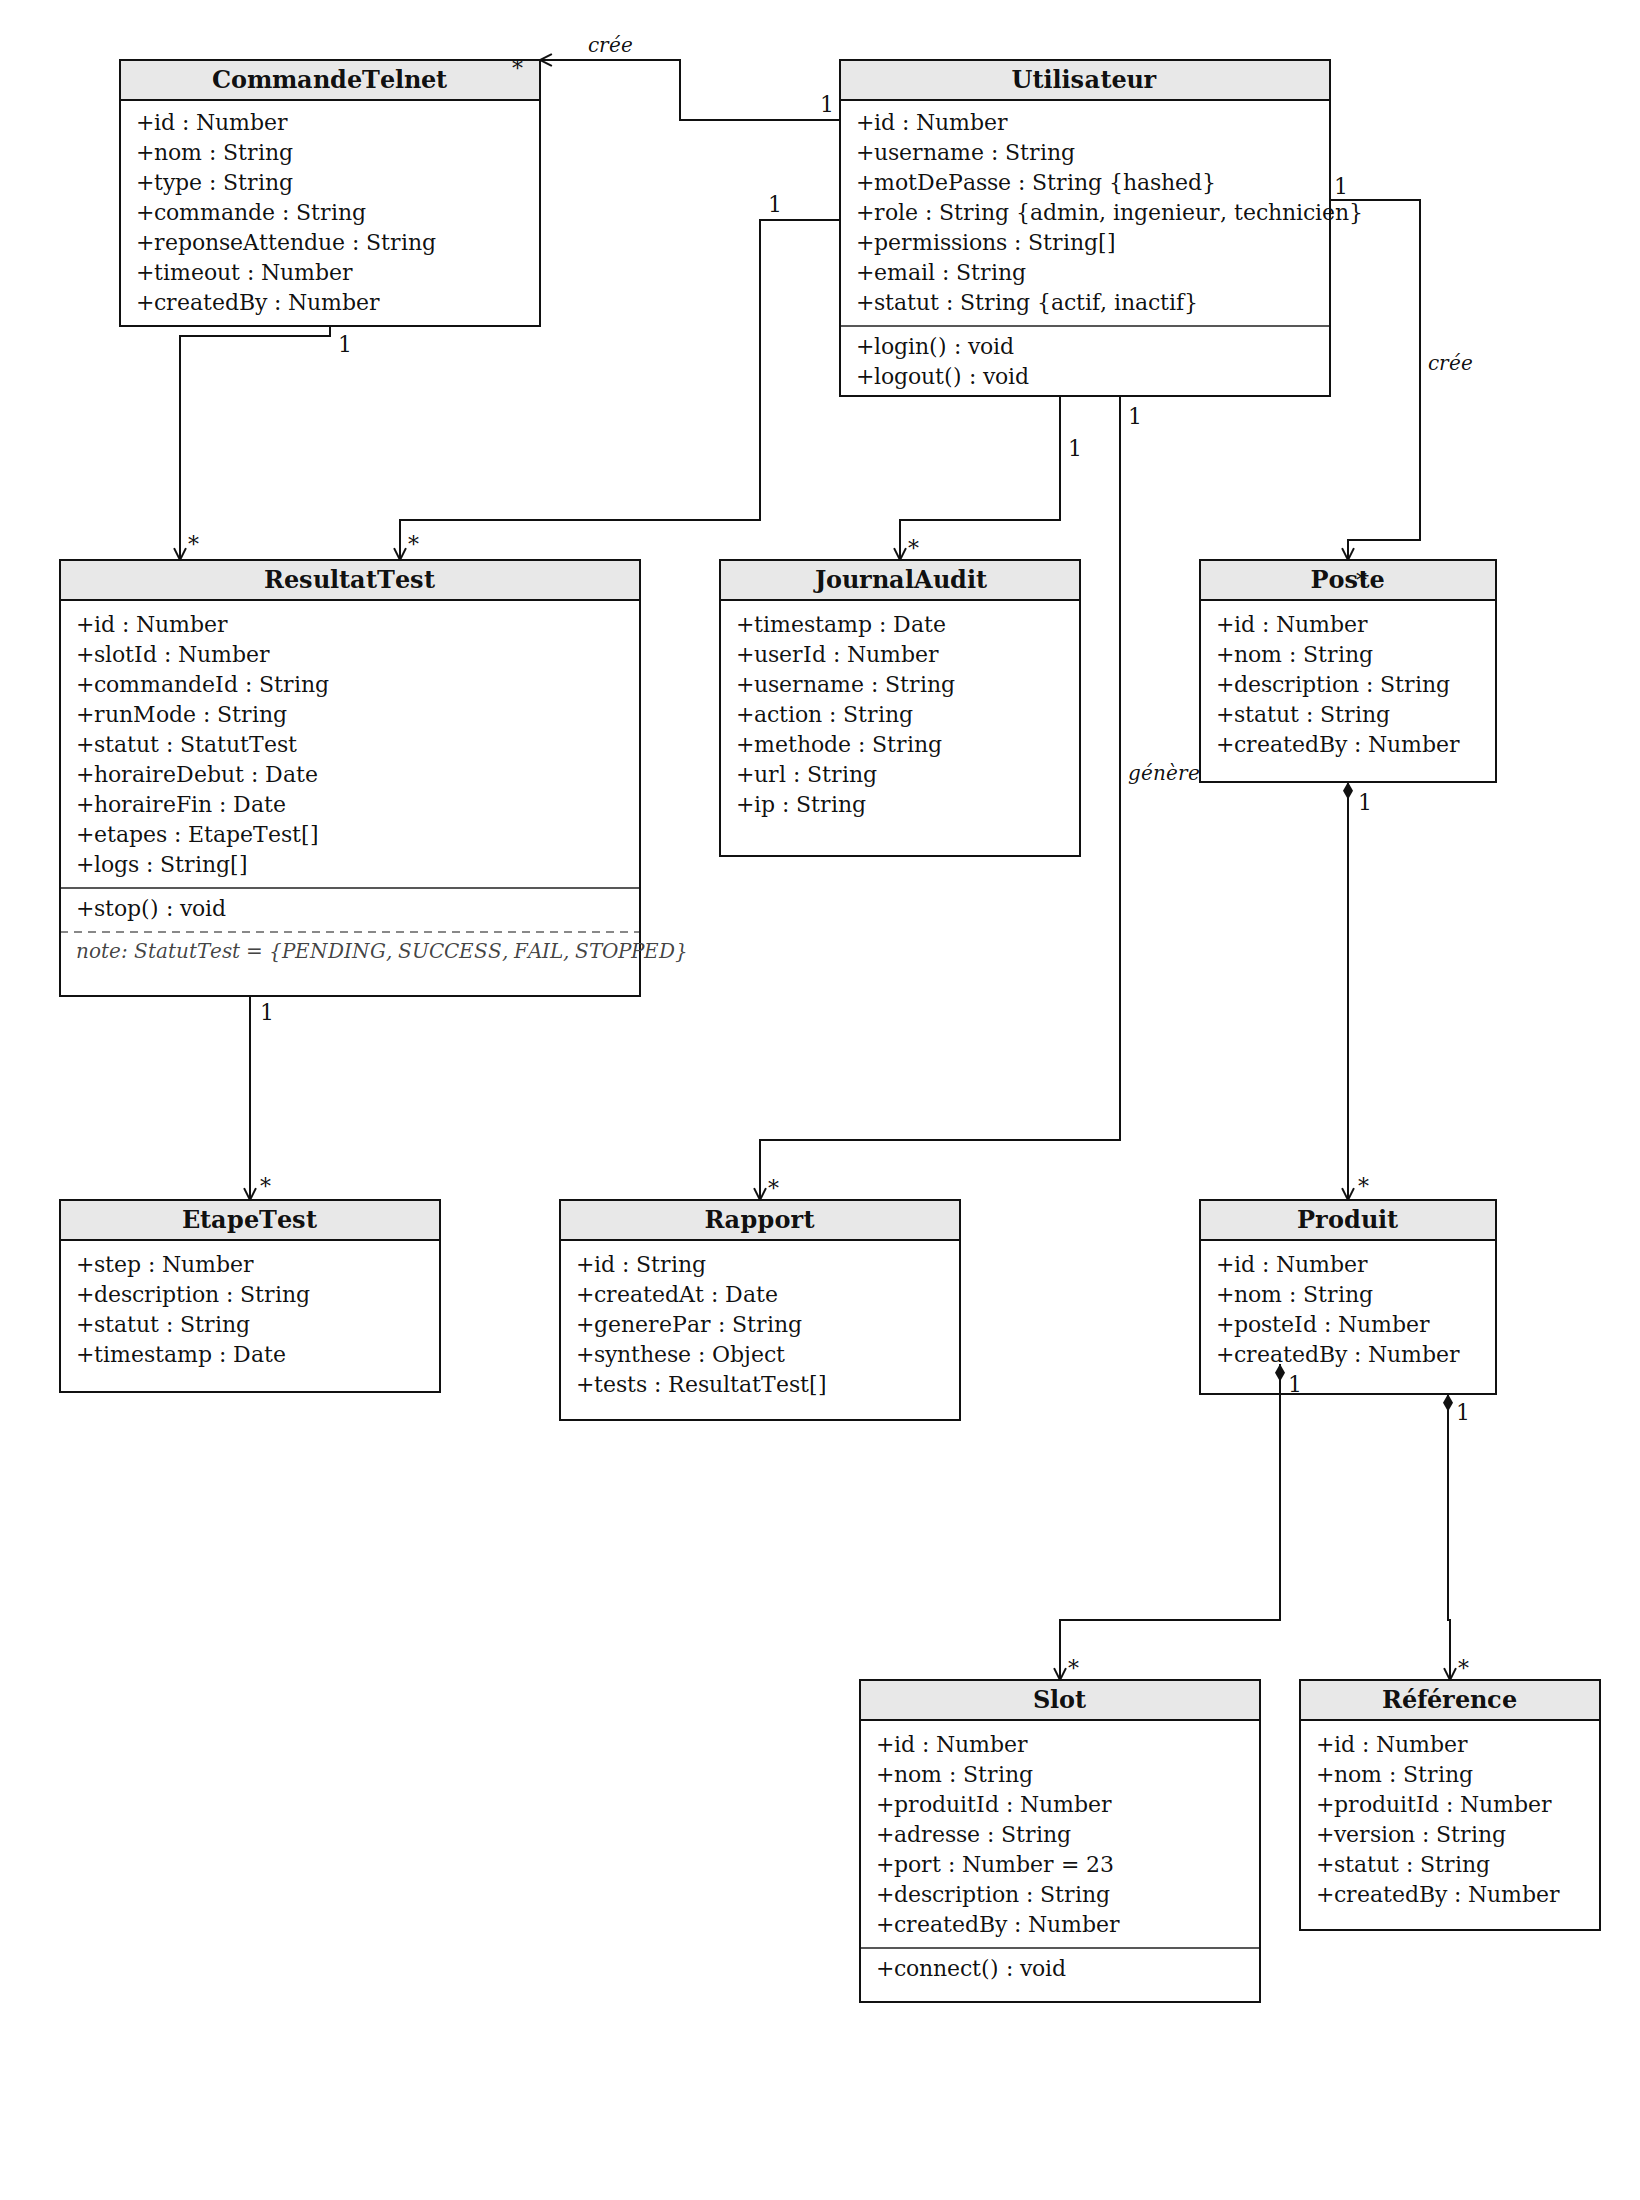
\includegraphics[width=\textwidth]{images/diagramclass}
  \caption{Diagramme de classes principal de Telnet Test Manager}
  \label{fig:class_diagram}
\end{figure}

% -----------------------------------------------------------------
\section{Diagrammes de séquence}
% -----------------------------------------------------------------

\subsection{Cas d'utilisation~: Authentification}

\begin{figure}[H]
  \centering
  \begin{tikzpicture}[
    life/.style={dashed,draw=gray!50},
    box/.style={draw=bleuPFE,fill=bleuPFE!8,minimum width=2.4cm,
                minimum height=0.6cm,align=center,font=\scriptsize},
    msg/.style={->,>=stealth,draw=bleuPFE,font=\scriptsize},
    ret/.style={->,>=stealth,draw=bleuPFE!50,dashed,font=\scriptsize},
    act/.style={draw=bleuPFE,fill=bleuPFE!20,minimum width=0.3cm,
                minimum height=1.2cm},
  ]

    % Participants
    \node[box] (user)  at (0,0)  {Utilisateur};
    \node[box] (front) at (3.5,0) {Frontend\\React};
    \node[box] (back)  at (7,0)  {Backend\\API};
    \node[box] (db)    at (10.5,0) {MongoDB};

    % Lifelines
    \draw[life] (0,-0.3) -- (0,-9);
    \draw[life] (3.5,-0.3) -- (3.5,-9);
    \draw[life] (7,-0.3) -- (7,-9);
    \draw[life] (10.5,-0.3) -- (10.5,-9);

    % Messages
    \draw[msg] (0,-1) -- (3.5,-1)
      node[midway,above,font=\scriptsize] {Saisie identifiants};
    \draw[msg] (3.5,-1.8) -- (7,-1.8)
      node[midway,above,font=\scriptsize] {\texttt{POST /login}};
    \draw[msg] (7,-2.6) -- (10.5,-2.6)
      node[midway,above,font=\scriptsize] {\texttt{findUser(username)}};
    \draw[ret] (10.5,-3.2) -- (7,-3.2)
      node[midway,above,font=\scriptsize] {User \{hash\}};
    \draw[msg] (7,-4) -- (7,-4)
      node[right,font=\scriptsize] {bcrypt.compare(mdp, hash)};
    \node[font=\scriptsize,color=gray,right] at (7.2,-4.7)
      {[succès] Génération JWT};
    \draw[ret] (7,-5.4) -- (3.5,-5.4)
      node[midway,above,font=\scriptsize]
      {200~: \{token, user\}};
    \draw[msg] (3.5,-6.2) -- (3.5,-6.2)
      node[right,font=\scriptsize]
      {Stockage token (sessionStorage)};
    \draw[ret] (3.5,-7) -- (0,-7)
      node[midway,above,font=\scriptsize] {Redirection Dashboard};

    % Fragment alt
    \draw[draw=bleuPFE!30,dashed] (1.5,-3) rectangle (9,-5);
    \node[font=\scriptsize\bfseries\color{bleuPFE!60}] at (2,-3.1)
      {[alt] Échec};
    \draw[ret] (7,-4.9) -- (3.5,-4.9)
      node[midway,above,font=\scriptsize] {401~: Identifiants invalides};

  \end{tikzpicture}
  \caption{Diagramme de séquence~: Authentification JWT}
  \label{fig:seq_auth}
\end{figure}

\subsection{Cas d'utilisation~: Exécution d'un test Telnet}

\begin{figure}[H]
  \centering
  \begin{tikzpicture}[
    life/.style={dashed,draw=gray!50},
    box/.style={draw=bleuPFE,fill=bleuPFE!8,minimum width=2.1cm,
                minimum height=0.6cm,align=center,font=\tiny},
    msg/.style={->,>=stealth,draw=bleuPFE,font=\tiny},
    ret/.style={->,>=stealth,draw=bleuPFE!50,dashed,font=\tiny},
  ]

    % Participants
    \node[box] (user)   at (0,0)    {Utilisateur};
    \node[box] (front)  at (2.5,0)  {Frontend};
    \node[box] (back)   at (5.5,0)  {Backend API};
    \node[box] (worker) at (8.5,0)  {Worker Thread};
    \node[box] (db)     at (11.2,0) {MongoDB};
    \node[box] (equip)  at (13.8,0) {Équipement\\TCP:23};

    % Lifelines
    \foreach \x in {0,2.5,5.5,8.5,11.2,13.8}
      \draw[life] (\x,-0.3) -- (\x,-13);

    % Messages
    \draw[msg] (0,-1)    -- (2.5,-1)
      node[midway,above] {Clic «Lancer le test»};
    \draw[msg] (2.5,-1.8) -- (5.5,-1.8)
      node[midway,above] {\texttt{POST /run-test}};
    \draw[msg] (5.5,-2.6) -- (5.5,-2.6)
      node[right] {Vérif. JWT \& permissions};
    \draw[msg] (5.5,-3.4) -- (11.2,-3.4)
      node[midway,above] {findSlot(slotId)};
    \draw[ret] (11.2,-4) -- (5.5,-4)
      node[midway,above] {Slot \{IP, port\}};
    \draw[msg] (5.5,-4.8) -- (11.2,-4.8)
      node[midway,above] {createTestResult (PENDING)};
    \draw[msg] (5.5,-5.6) -- (8.5,-5.6)
      node[midway,above] {spawnWorker(testId, slot, cmd)};
    \draw[ret] (5.5,-6.2) -- (2.5,-6.2)
      node[midway,above] {200~: \{testId\}};
    \draw[ret] (2.5,-6.9) -- (0,-6.9)
      node[midway,above] {Affichage «En cours...»};

    % Worker
    \draw[msg] (8.5,-7.7) -- (13.8,-7.7)
      node[midway,above] {Connexion TCP port 23};
    \draw[msg] (8.5,-8.4) -- (13.8,-8.4)
      node[midway,above] {Authentification (login/mdp)};
    \draw[msg] (8.5,-9.1) -- (13.8,-9.1)
      node[midway,above] {Envoi commande Linux};
    \draw[ret] (13.8,-9.8) -- (8.5,-9.8)
      node[midway,above] {Réponse Telnet};
    \draw[msg] (8.5,-10.5) -- (8.5,-10.5)
      node[right] {Comparaison expectedResponse};
    \draw[msg] (8.5,-11.2) -- (5.5,-11.2)
      node[midway,above] {WS~: \{step, status\}};
    \draw[msg] (5.5,-11.2) -- (2.5,-11.2);
    \draw[ret] (2.5,-11.2) -- (0,-11.2)
      node[midway,above] {Mise à jour UI (temps réel)};
    \draw[msg] (8.5,-12) -- (11.2,-12)
      node[midway,above] {updateTestResult (SUCCESS)};

  \end{tikzpicture}
  \caption{Diagramme de séquence~: Exécution d'un test Telnet}
  \label{fig:seq_telnet}
\end{figure}

\subsection{Cas d'utilisation~: Gestion CRUD des équipements}

\begin{figure}[H]
  \centering
  \begin{tikzpicture}[
    life/.style={dashed,draw=gray!50},
    box/.style={draw=bleuPFE,fill=bleuPFE!8,minimum width=2.4cm,
                minimum height=0.6cm,align=center,font=\scriptsize},
    msg/.style={->,>=stealth,draw=bleuPFE,font=\scriptsize},
    ret/.style={->,>=stealth,draw=bleuPFE!50,dashed,font=\scriptsize},
  ]
    \node[box] (ing)   at (0,0)    {Ingénieur};
    \node[box] (front) at (3.5,0)  {Frontend\\React};
    \node[box] (back)  at (7,0)    {Backend\\API};
    \node[box] (db)    at (10.5,0) {MongoDB};

    \draw[life] (0,-0.3)    -- (0,-9);
    \draw[life] (3.5,-0.3)  -- (3.5,-9);
    \draw[life] (7,-0.3)    -- (7,-9);
    \draw[life] (10.5,-0.3) -- (10.5,-9);

    \draw[msg] (0,-1)    -- (3.5,-1)
      node[midway,above] {Clic «Ajouter un poste»};
    \draw[ret] (3.5,-1.8) -- (0,-1.8)
      node[midway,above] {Affichage formulaire modal};
    \draw[msg] (0,-2.6)  -- (3.5,-2.6)
      node[midway,above] {Saisie nom + description};
    \draw[msg] (3.5,-3.4) -- (7,-3.4)
      node[midway,above] {\texttt{POST /postes \{nom, desc\}}};
    \draw[msg] (7,-4.2)  -- (7,-4.2)
      node[right] {Vérif. JWT + rôle Ingénieur};
    \draw[msg] (7,-5)    -- (10.5,-5)
      node[midway,above] {\texttt{PosteRepo.create(poste)}};
    \draw[ret] (10.5,-5.7) -- (7,-5.7)
      node[midway,above] {\{id: N, nom, createdAt\}};
    \draw[ret] (7,-6.5)  -- (3.5,-6.5)
      node[midway,above] {201~: poste créé};
    \draw[msg] (3.5,-7.3) -- (3.5,-7.3)
      node[right] {Actualise la liste};
    \draw[ret] (3.5,-8.1) -- (0,-8.1)
      node[midway,above] {Notification «Succès»};

    \draw[draw=bleuPFE!25,dashed] (1.5,-6) rectangle (5,-8.7);
    \node[font=\scriptsize\bfseries\color{bleuPFE!60}] at (2.1,-6.1)
      {[alt] PUT/DELETE};
  \end{tikzpicture}
  \caption{Diagramme de séquence~: Création d'un équipement (CRUD)}
  \label{fig:seq_crud}
\end{figure}

\subsection{Cas d'utilisation~: Tests multi-slots en parallèle}

\begin{figure}[H]
  \centering
  \begin{tikzpicture}[
    life/.style={dashed,draw=gray!50},
    box/.style={draw=bleuPFE,fill=bleuPFE!8,minimum width=1.8cm,
                minimum height=0.6cm,align=center,font=\tiny},
    msg/.style={->,>=stealth,draw=bleuPFE,font=\tiny},
    ret/.style={->,>=stealth,draw=bleuPFE!50,dashed,font=\tiny},
  ]
    \node[box] (ing)   at (0,0)    {Ingénieur};
    \node[box] (front) at (2.5,0)  {Frontend};
    \node[box] (back)  at (5.5,0)  {Backend};
    \node[box] (w1)    at (8.5,0)  {Worker 1\\(Slot A)};
    \node[box] (w2)    at (11,0)   {Worker 2\\(Slot B)};
    \node[box] (db)    at (13.5,0) {MongoDB};

    \foreach \x in {0,2.5,5.5,8.5,11,13.5}
      \draw[life] (\x,-0.3) -- (\x,-13.5);

    \draw[msg] (0,-1) -- (2.5,-1)
      node[midway,above] {Sélection 2 slots + commande};
    \draw[msg] (2.5,-1.8) -- (5.5,-1.8)
      node[midway,above] {\texttt{POST /run-test \{slotIds:[A,B]\}}};
    \draw[msg] (5.5,-2.6) -- (13.5,-2.6)
      node[midway,above] {createTestResults ×2 (PENDING)};
    \draw[msg] (5.5,-3.4) -- (8.5,-3.4)
      node[midway,above] {spawnWorker(id1, slotA)};
    \draw[msg] (5.5,-4)   -- (11,-4)
      node[midway,above] {spawnWorker(id2, slotB)};
    \draw[ret] (5.5,-4.8) -- (2.5,-4.8)
      node[midway,above] {200~: \{testIds:[1,2]\}};
    \draw[ret] (2.5,-5.4) -- (0,-5.4)
      node[midway,above] {Affiche «En cours (×2)»};

    \draw[draw=bleuPFE!25,dashed] (6,-6.2) rectangle (14.5,-12.5);
    \node[font=\tiny\bfseries\color{bleuPFE!60}] at (7.2,-6.3)
      {par (parallèle)};

    \draw[msg] (8.5,-6.8)  -- (8.5,-6.8)  node[right] {TCP SlotA:23 + auth + cmd};
    \draw[msg] (8.5,-7.5)  -- (5.5,-7.5)  node[midway,above] {WS~: step SUCCESS};
    \draw[msg] (8.5,-8.2)  -- (13.5,-8.2) node[midway,above] {updateResult (SUCCESS)};

    \draw[msg] (11,-9.2)   -- (11,-9.2)   node[right] {TCP SlotB:23 + auth + cmd};
    \draw[msg] (11,-9.9)   -- (5.5,-9.9)  node[midway,above] {WS~: step FAIL};
    \draw[msg] (11,-10.6)  -- (13.5,-10.6)node[midway,above] {updateResult (FAIL)};

    \draw[msg] (5.5,-11.5) -- (2.5,-11.5)
      node[midway,above] {WS broadcast résultats finals};
    \draw[ret] (2.5,-12.3) -- (0,-12.3)
      node[midway,above] {UI~: SUCCESS/FAIL par slot};

  \end{tikzpicture}
  \caption{Diagramme de séquence~: Tests multi-slots en parallèle}
  \label{fig:seq_multislot}
\end{figure}

\subsection{Cas d'utilisation~: Génération de rapport}

\begin{figure}[H]
  \centering
  \begin{tikzpicture}[
    life/.style={dashed,draw=gray!50},
    box/.style={draw=bleuPFE,fill=bleuPFE!8,minimum width=2.4cm,
                minimum height=0.6cm,align=center,font=\scriptsize},
    msg/.style={->,>=stealth,draw=bleuPFE,font=\scriptsize},
    ret/.style={->,>=stealth,draw=bleuPFE!50,dashed,font=\scriptsize},
  ]
    \node[box] (ing)   at (0,0)    {Ingénieur};
    \node[box] (front) at (3.5,0)  {Frontend\\React};
    \node[box] (back)  at (7,0)    {Backend\\API};
    \node[box] (db)    at (10.5,0) {MongoDB};

    \draw[life] (0,-0.3)    -- (0,-9.5);
    \draw[life] (3.5,-0.3)  -- (3.5,-9.5);
    \draw[life] (7,-0.3)    -- (7,-9.5);
    \draw[life] (10.5,-0.3) -- (10.5,-9.5);

    \draw[msg] (0,-1)    -- (3.5,-1)
      node[midway,above] {Filtre par date, statut, slot};
    \draw[msg] (3.5,-1.8) -- (7,-1.8)
      node[midway,above] {\texttt{POST /reports/generate \{filters\}}};
    \draw[msg] (7,-2.6)  -- (10.5,-2.6)
      node[midway,above] {findTestResults(filters)};
    \draw[ret] (10.5,-3.3) -- (7,-3.3)
      node[midway,above] {Liste résultats filtrés};
    \draw[msg] (7,-4.1)  -- (7,-4.1)
      node[right] {Calcul synthèse (taux succès, durée moy.)};
    \draw[msg] (7,-4.9)  -- (10.5,-4.9)
      node[midway,above] {RapportRepo.create(rapport)};
    \draw[ret] (10.5,-5.6) -- (7,-5.6)
      node[midway,above] {\{id, createdAt\}};
    \draw[ret] (7,-6.4)  -- (3.5,-6.4)
      node[midway,above] {201~: rapport complet};
    \draw[msg] (3.5,-7.2) -- (3.5,-7.2)
      node[right] {Affiche rapport + statistiques};
    \draw[ret] (3.5,-8)  -- (0,-8)
      node[midway,above] {Rapport affiché};
    \draw[msg] (0,-8.8)  -- (3.5,-8.8)
      node[midway,above] {[opt] Clic «Exporter»};

  \end{tikzpicture}
  \caption{Diagramme de séquence~: Génération d'un rapport}
  \label{fig:seq_rapport}
\end{figure}

% -----------------------------------------------------------------
\section{Modèle de la base de données MongoDB}
% -----------------------------------------------------------------

\subsection{Justification du choix NoSQL}

MongoDB a été choisi pour plusieurs raisons pratiques~:
\begin{itemize}
  \item Le \textbf{schéma flexible} s'adapte aux données de tests dont
        la structure varie selon le type de test (étapes, logs)~;
  \item Les opérations en \textbf{lecture/écriture intensive} sur les
        journaux d'audit sont bien gérées~;
  \item La sérialisation native en \textbf{BSON/JSON} s'intègre
        naturellement dans l'écosystème Node.js~;
  \item L'intégration avec \textbf{Mongoose} (ODM) est simple et apporte
        validation de schéma et middlewares.
\end{itemize}

% -----------------------------------------------------------------
\section{Conception des interfaces utilisateur}
% -----------------------------------------------------------------

\subsection{Tableau de bord principal (Dashboard)}

Le tableau de bord regroupe la sélection et l'exécution des tests en
une seule page. Il comprend~:
\begin{itemize}
  \item Un panneau de sélection hiérarchique (Poste~$\to$ Produit~$\to$
        Slot) permettant d'identifier l'équipement cible~;
  \item Un sélecteur de commandes Telnet avec prévisualisation des étapes~;
  \item Un terminal de résultats en temps réel (mise à jour par WebSocket)
        affichant chaque étape avec son statut et son horodatage~;
  \item Des boutons d'action~: Lancer, Arrêter, Exporter.
\end{itemize}


\subsection{Module de configuration}

L'interface de configuration présente les données en \textbf{tableaux}
avec des formulaires modaux pour les opérations CRUD. La hiérarchie
Poste~$\to$ Produit~$\to$ Slot~$\to$ Référence se navigue par onglets.


\subsection{Panneau d'administration}

Le panneau d'administration comprend cinq onglets~:
\begin{enumerate}
  \item \textbf{Vue d'ensemble}~: métriques globales (utilisateurs actifs,
        tests du jour, taux de succès)~;
  \item \textbf{Gestion des utilisateurs}~: tableau \gls{crud} avec
        assignation de rôles et permissions~;
  \item \textbf{Historique des tests}~: tous les tests de tous les
        utilisateurs, filtrables~;
  \item \textbf{Journal d'audit}~: liste chronologique des actions avec
        filtrage par utilisateur, action et date~;
  \item \textbf{Analytiques}~: graphiques de répartition des tests par
        statut, utilisateur et période.
\end{enumerate}


\section*{Conclusion}

Ce chapitre a défini les choix d'architecture et de conception du projet.
L'architecture N-tiers combinée à la Clean Architecture assure la
séparation des responsabilités et facilite les tests. Les diagrammes de
classes et de séquence décrivent les interactions entre composants. Le
chapitre suivant détaille la mise en œuvre technique de ces choix.
